\documentclass[pra,aps,superscriptaddress,amssymb,amsmath,reprint,noeprint,floatfix]{revtex4-2}

\usepackage{natbib}
\usepackage{braket}
\usepackage{bm}
% \usepackage[margin=3.0cm]{geometry} 
\usepackage{algorithm}
\usepackage{algpseudocode}
\usepackage{graphicx}
\usepackage{xcolor}
\usepackage[colorlinks = true,
            linkcolor = red,
            urlcolor  = red,
            citecolor = red,
            anchorcolor = red]{hyperref}
\hypersetup{bookmarksnumbered}


\bibliographystyle{apsrev4-2}

\begin{document}

\title{AP3082 Project 2: Ising Model}
\date{\today}

\author{Kah Jen Wo}
\affiliation{Faculty of Applied Sciences, Delft University of Technology, Delft, The Netherlands}
\author{Juan Torres}
\affiliation{Faculty of Applied Sciences, Delft University of Technology, Delft, The Netherlands}

\begin{abstract}
    Two different algorithms have been employed in studying the 2D square lattice Ising model numerically. The two algorithms used in this study are the Metropolis algorithm and the Wolff algorithm. We verify the validity of our simulation results by comparing the numerical observables obtained with the analytical behaviour. We access the difference in the observables produced by each of the algorithm by means of investigating the errors produced by each of the algorithms.
\end{abstract}
\maketitle

\section{\label{sec:introduction}Introduction}
The Ising model is a nearest-neighbour spin interaction model used to describe ferromagnetism in metals by using discrete binary variables and it has been used to study phase transitions in finite substances such as iron and nickel where ferromagnetism spontaneously arise when cooled below a certain critical temperature, i.e.\ the Curie temperature.

The model was first introduced by Ernst Ising in an attempt to describe phase transition in ferromagnetic substances \cite{1925ZPhy...31..253I}. His attempt has proved that ferromagnets in 1D disappointingly do not exhibit phase transitions. Since then, many have made an effort into obtaining a more accurate understanding of the model. In 1943, it was then shown analytically by Lars Onsager that phase transition in 2D Ising model is indeed possible \cite{PhysRev.65.117}. The Ising model is now being utilised in various fields such as machine learning to extract insights from complex physical systems \cite{Walker2020}. 

In statistical mechanics, the properties of a time-dependent evolving many-body system are calculated as an average over an emsemble of the system under certain constraints. It requires several approximations such as infinitely large domain to obtain insights into the physics of the system. Nevertheless, these insights have proved invaluable in the scientific community's attempt to understand the Ising model in detail. For example, Ising model has provided an accurate description of FeCO$_3$ and FeCl$_2$, which are anisotropic crystals \cite{diu1989elements}.

Unfortunately, these approximations do not apply in practice because systems with infinite domain do not exist. This is the reason why computational approach is needed: to recover the properties of the system from the statistical behaviour of an arbitrarily sized simulation domain. Numerical approaches, however, still present their own set of challenges such as computational efficiency, accuracy and limitations due to lack of computational resources.

In a classical Ising model, the computational approach to simulate the system is by means of \textit{Monte-Carlo} procedures. Monte Carlo simulations often see a Metropolis-type update mechanism, which is also known as Metropolis algorithm \cite{doi:10.1063/1.1699114}. This algorithm involves flipping single spins at each iteration and is considered simple. More recently, cluster algorithms were invented, such as the one by Ulli Wolff, which is now known as the Wolff algorithm \cite{wolff_algo}. There are more modern and advanced algorithms which exist today for the purpose of simulating Ising model systems. However, in this paper, we will study the Ising model using only the Metropolis and Wolff algorithm.

We begin with the review of relevant background theory in Ising model in section \ref{sec:backgroundtheory} which is used in our study of the classical 2D Ising model. In section \ref{sec:algorithms}, we discuss the Metropolis and Wolff algorithm and provide the pseudocode for each of these algorithms. In section \ref{sec:ErgodicityandDetailedbalance}, we discuss the important criteria which our simulation should meet. In section \ref{sec:resultsanddiscussion}, we present our results from the simulations from both algorithms as well as their corresponding discussions. Finally, in section \ref{sec:conclusion}, we provide the conclusion of our study.

\section{\label{sec:backgroundtheory}Background theory for Ising model}
In this section we review the relevant theories in Ising model for our simulations.

\subsection{\label{subsec:hamiltonian}Nearest neighbour Hamiltonian}
Consider a ferromagnetic 2D square lattice Ising model, where the $i^\mathrm{th}$ spin in the lattice is denoted by $S_i$ and each of them can either spin down or spin up along the $z$-axis, i.e.\ $S_i\in\{-1,1\}$. Its Hamiltonian is modelled as such
\begin{equation}\label{eqn:hamltonian}
    H=-J\sum_{\braket{i,j}} S_iS_j-h\sum_{i=1}^{N} S_i
\end{equation}
where $J$ is a positive ferromagnetic coupling constant, $\braket{i,j}$ denotes sum over all nearest neighbour pairs without double counting, $h$ is the strength of the external magnetic field along the $z$-axis, and $N=L\times L$ is the total number of sites on the square lattice.

\subsection{\label{subsec:phasetransition}Phase transition}
In Ising model there are two distinct phases: \textit{paramagnetic} phase and \textit{ferromagnetic} phase. In paramagnetic phase, the spins take on random direction and are disordered due to high thermal fluctuations, i.e.\ average magnetisation of zero. In ferromagnetic phase, the spins are more likely to align with a certain direction. In this section, we review the critical temperature $T_C$, below which the Ising model system takes on the ferromagnetic phase and above which takes on the paramagnetic phase.


The phase transition of the system can be studied using the physical observables shown in section \ref{subsec:observables}. The most common observable used to determine the critical temperature of the system is the magnetisation, where its expression is given in Eqn.\ \ref{eqn:magnetisation}. The average magnetisation is used to represent the \textit{order parameter}. In mean field theory, the critical temperature $T_C$ for the 2D ising model was estimated to be $4J/k_B$. However, in mean field theory we assume that fluctuations are small and thus it tends to overestimates the value of $T_C$. 

Fortunately, the exact analytical expression for the magnetisation of the 2D square lattice Ising model for $T<T_C$ has been obtained by Kramers and Wannier \cite{PhysRev.60.252}:
\begin{equation}\label{eqn:analmagnetisation}
    M=\left(1-\sinh^{-4}{(2\beta J)}\right)^{1/8}
\end{equation}
Solving for $M=0$ in Eqn.\ \ref{eqn:analmagnetisation} yields the exact critical temperature, which we will use in our simulation. That is $T_C=\frac{2J}{k_B \ln{\left(1+\sqrt{2}\right)}}\approx2.27J/k_B$.

In Fig.\ \ref{fig:FreeEnergy}, we see the free energy diagram of the Ising model system for varying temperature and magnetisation when there is no external magnetic field. From the temperature axis, we see that when $T=T_C$, the free energy transitions from having two minimas to having one minima. The figure also shows that in the ferromagnetic phase ($T<T_C$), the spins prefer either a spin down or spin up configuration while in the paramagnetic phase ($T>T_C$), the spins do not have a preference for any configuration, leading to zero average magnetisation.
\begin{figure}
    \centering
    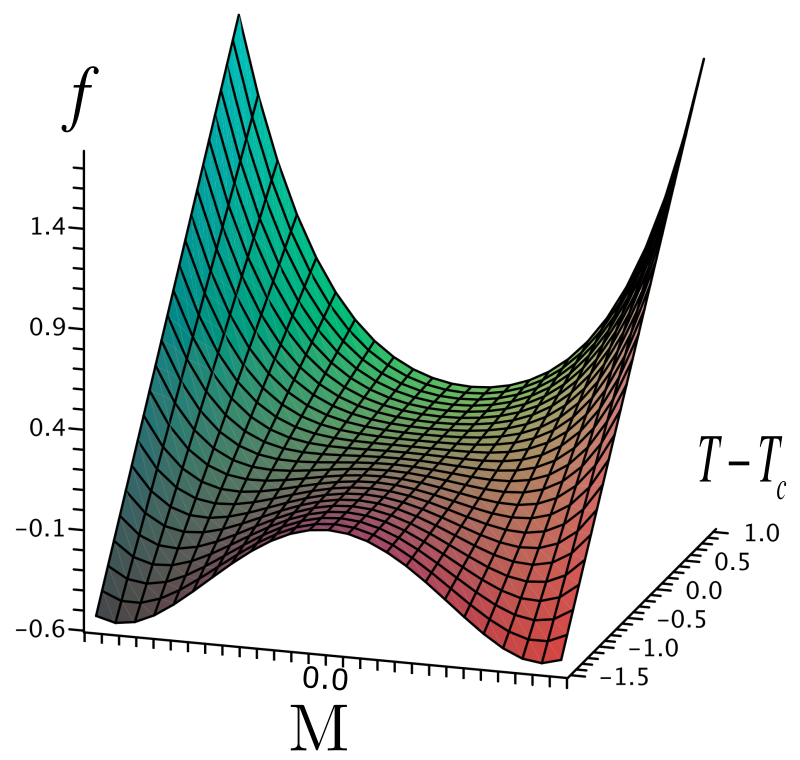
\includegraphics[width=0.5\linewidth]{Figures/ising_model_free_energy.png}
    \caption{Free energy (denoted by $f$ in the vertical axis) of a Ising model system for varying magnetisation $M$ and temperature $T$. The external magnetic field is zero. Source: Adapted from \cite{ProvatasTextbook}.}
    \label{fig:FreeEnergy}
\end{figure}

\subsection{\label{subsec:observables}Physical observables}
The observable quantities are imperative in aiding the study of thermodynamic properties in the Ising model. One of these quantities is the average \textit{magnetisation}
\begin{equation}\label{eqn:magnetisation}
    \braket{M}=\frac{1}{N}\sum^{N}_{i=1} \braket{S_i}
\end{equation}
The specific heat per spin
\begin{equation}\label{eqn:specificheat}
    c=\frac{k_B\beta^2}{N}\left(\braket{E^2}-\braket{E}^2\right)
\end{equation}
The susceptibility per spin
\begin{equation}\label{eqn:susceptibility}
    \chi=\beta N \left(\braket{M^2}-\braket{M}^2\right)
\end{equation}
where $\beta=\frac{1}{k_BT}$, $k_B$ is the Boltzmann constant and $T$ is the temperature.

\section{\label{sec:algorithms}Monte Carlo Algorithms}
In this section we review two different algorithms that we used in our study of the 2D square lattice Ising model.
\subsection{\label{subsec:metropolis}Metropolis algorithm}
It is worth noting that even though the Metropolis algorithm seems relatively simple, it has been met with considerable amount of success when it comes to generating data of the physical observables in systems that exhibit Ising-like model, e.g. model mono-layer of nano-graphene with the presence of an external magnetic field \cite{IVASHKO2019165617}. Below there is the pseudo-code for a single iteration of Metropolis algorithm.
%For example, it has been used to model the ferromagnetism of a mono-layer of nano-graphene with the presence of an external magnetic field \cite{IVASHKO2019165617}. Below, we find the pseudo-code for \textbf{one iteration} in the Metropolis algorithm.
\begin{algorithm}[H]
    \caption{Metropolis}
    \begin{algorithmic}[1]
        \State Calculate $E_\mathrm{current}$.
        \State Choose a random spin to flip with uniform distribution.
        \State Calculate $E_\mathrm{trial}$.
        \State Calculate $\Delta E=E_\mathrm{current}-E_\mathrm{trial}$.
        \If {$\Delta E \leq0$}
            \State Set $E_\mathrm{current}=E_\mathrm{trial}$.
        \Else 
            \State Choose a random number $r\in(0,1)$ with uniform distribution.
            \State Compute $W=e^{-\frac{\Delta E}{k_BT}}$.
            \If {$r<W$}
                \State Set $E_\mathrm{current}=E_\mathrm{trial}$.
            \Else
                \State Do nothing. (i.e.\ the lattice stays the same)
            \EndIf
        \EndIf
    \end{algorithmic}
    \label{alg:metropolis}
\end{algorithm}
\subsection{\label{subsec:Wolff}Wolff algorithm}
Instead of flipping a single spin at each iteration as shown in the Metropolis algorithm, the Wolff algorithm flips an entire \textit{cluster}. It should also be noted that the Wolff algorithm does not take external magnetic field into account, so we can only simulate Ising model with $h=0$. Below, we find the pseudo-code for \textbf{one iteration} in the Wolff algorithm.
\begin{algorithm}[H]
    \caption{Wolff}
    \begin{algorithmic}[1]
        \State Choose a random spin as the seed with uniform distribution.
        \State Check the neighbours of the seed spin. 
        \State If they have the same direction as that spin, add them to the cluster with probability $P_\mathrm{add}=1-e^{-\frac{2J}{k_BT}}$.
        \State For each added spin from the previous step, repeat step 3 until there are no spins left in the cluster whose neighbours have not been considered for inclusion in the cluster.
        \State Flip the cluster.
    \end{algorithmic}
    \label{alg:wolff}
\end{algorithm}

\section{\label{sec:ErgodicityandDetailedbalance}Ergodicity and detailed balance}
It is imperative that the Monte Carlo algorithms satisfy the following criteria \cite{newman1999monte}:
\begin{enumerate}
    \itemsep-0.32em
    \item It should be possible for the state of the system from a configuration $a$ lead to a configuration $b$ such that all configurations in phase space are reached if we run it for long enough. This is a must to generate states for correct Boltzmann probabilities. (\textbf{Ergodicity})
    \item For a long enough simulation, the probability distribution that the equilibrated system generates must be the Boltzmann probability distribution. (\textbf{Detailed balance})
\end{enumerate}
It is interesting to note that for local algorithms such as Metropolis algorithm (given in section \ref{subsec:metropolis}), they fulfil the criteria for the most part in Ising model but fail when the system is near the criticality regime. This is due to the algorithm implementing too small of a change in the magnetisation in one iteration while there is a wide distribution of magnetisation, i.e.\ there are regions of the same spin which are difficult for the Metropolis algorithm to flip. Hence, cluster algorithms such as the Wolff algorithm was developed as a solution to this problem, which is given in section \ref{subsec:Wolff}.

\section{\label{sec:resultsanddiscussion}Results and discussion}
To study physical quantities from a simulation with a statistical nature, a systematic study of different system parameters is given. First, a study of the convergence of the system towards the expected behaviour as a function of system size and number of relaxation steps is presented for both algorithms. Once a criteria for significant results is established, a derivation of three physical quantities is presented, i.e.\ magnetisation, specific heat and magnetic susceptibility. The three critical exponents associated to these quantities are presented. Similarly, the full range of parameters is studied in a phase diagram. Finally, a discussion about the performance of the code is presented.

\subsection{\label{subse:errors}Error calculation}
Two kinds of errors will be discussed. On one hand, errors obtained by comparison with exact analytical expression derived for the 2D Ising model \cite{PhysRev.65.117}. On the other hand, statistical errors induced by correlations in the data sets due to the nature of the algorithms used. To describe the statistical errors, the autocorrelation function of a given data set is calculated, and the correlation time $\tau$ is extracted from it. The autocorrelation function of observable $A$ is given as,
\begin{equation}
    \chi_A(t) = \frac{(N-t)\sum_n A_nA_{n+t}-\sum_nA_n\sum_nA_{n+t}}{\sigma_n\sigma_{n+t}},
\end{equation}
where $\sigma_n = \sqrt{(N-t)\sum_nA_n^2-(\sum_nA_n)^2}$, and $N$ is the length of the data set. Errors are calculated using the block data method \cite{newman1999monte}. First, the data set is divided into uncorrelated groups separated by a distance $\tau$. Each block is then converted into a single value that corresponds to the mean of the block, and its error corresponds to the standard deviation of the data inside the block. In Fig.\ \ref{fig:taus} one can observe that the correlation length increases with the system size for the Metropolis algorithm. That is, correlation increases with system size. On the other hand, for the Wolff algorithm it always remains much smaller. From these results, one can expect a priori to have smaller errors for the Wolff algorithm.
\begin{figure}[H]
    \centering
    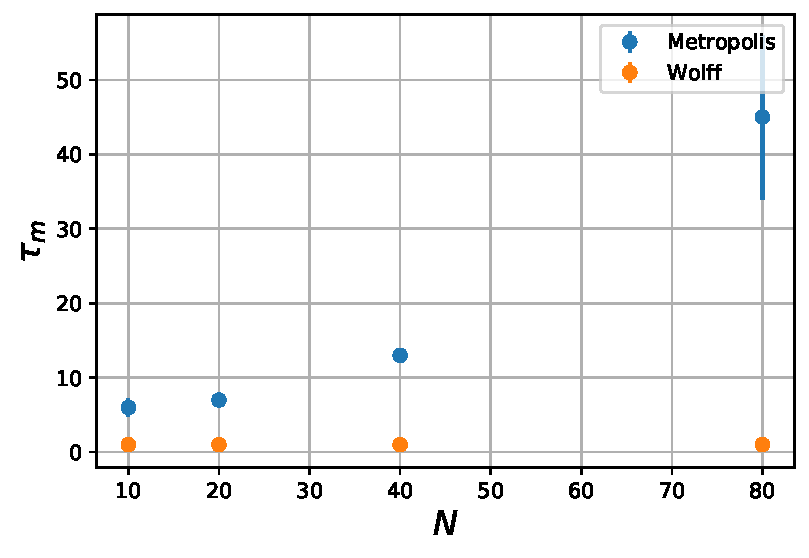
\includegraphics[width=0.8\linewidth]{Figures/taus_m.pdf}
    \caption{Correlation time versus system size for the Metropolis and Wolff algorithms. These results correspond to the ones shown in Fig. \ref{fig:size_dep}.}
    \label{fig:taus}
\end{figure}
\subsection{\label{subsec:systemsizedependence}System size dependence}
An exact solution for the Ising model was derived by Onsager \cite{PhysRev.65.117} for the case of an infinite system. In a finite system, we converge towards the exact result as the system size increases. In Fig.\ \ref{fig:size_dep} we can observe the behaviour of the magnetisation as a function of the temperature for different system sizes. 

\begin{figure}[H]
    \centering
    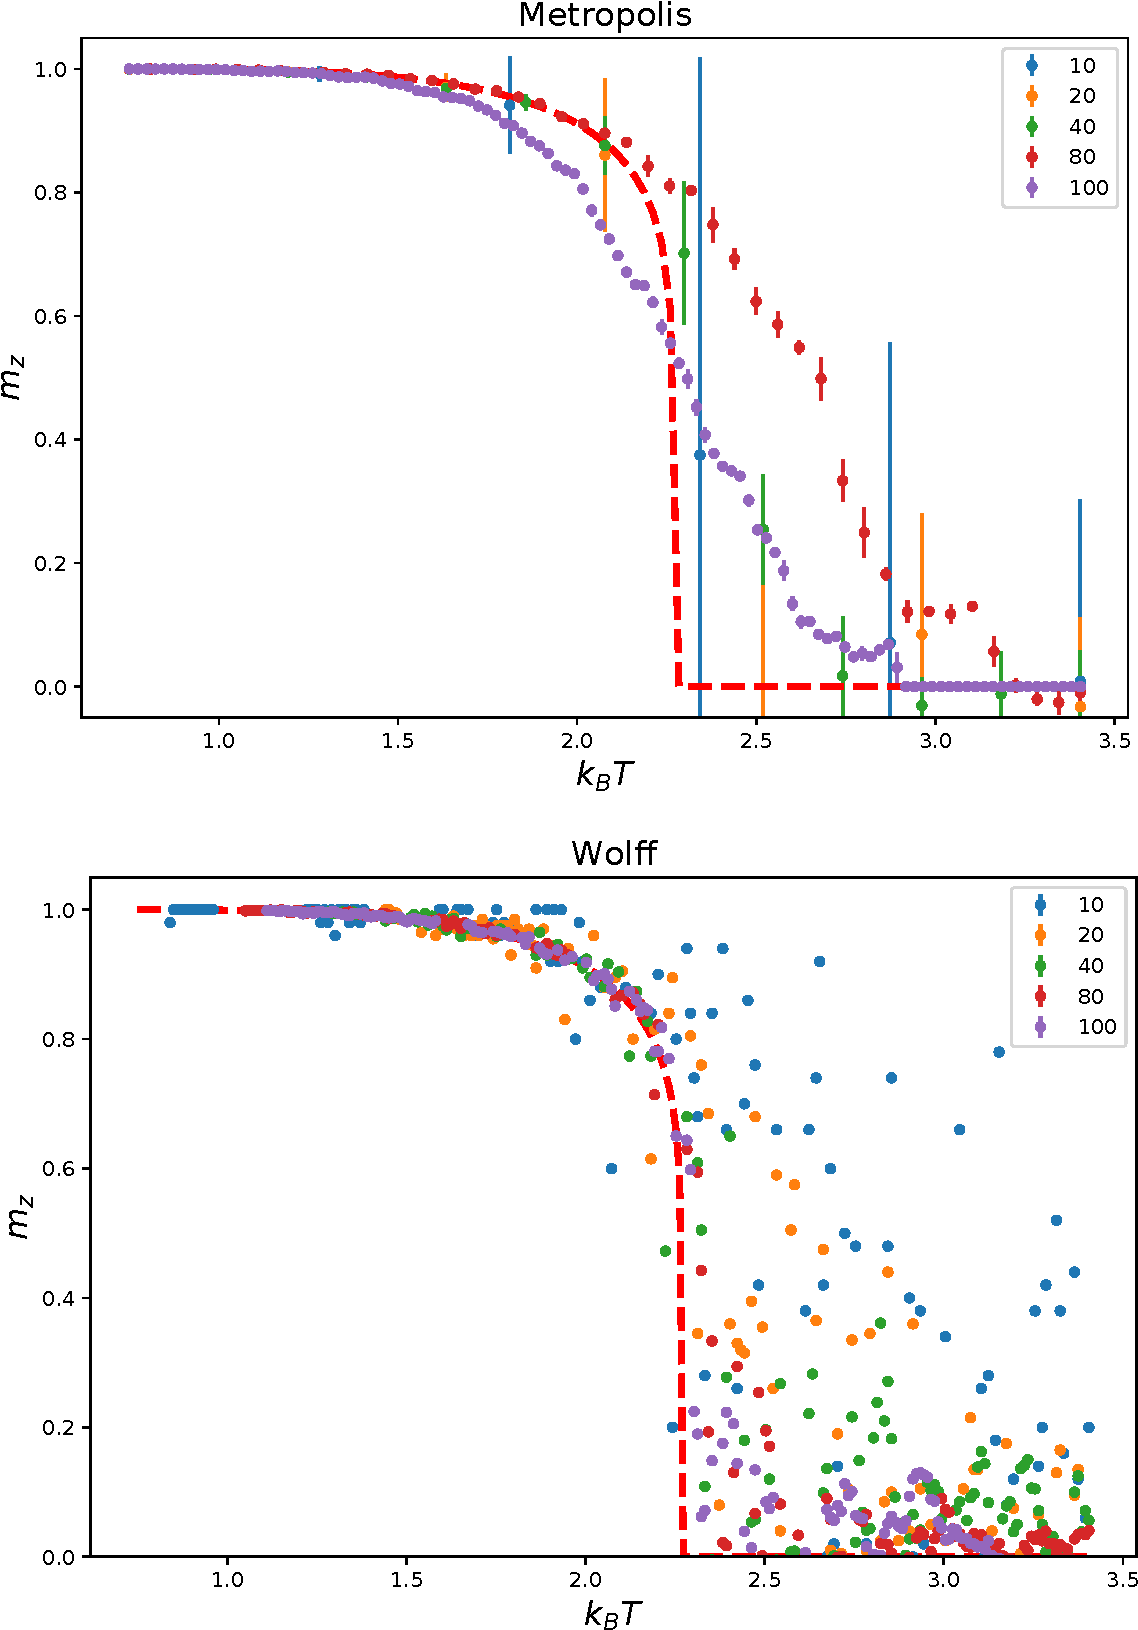
\includegraphics[width=0.8\linewidth]{Figures/size_dependence.pdf}
    \caption{Magnetisation with respect to temperature. Here $k_B=1$, $J=1$ and $h=0$. Red dashed curve corresponds to exact analytical result for an infinite system. Different curves correspond to different system sizes, i.e. $N$. Both cases were evaluated for $265$ points. Data was further decreased by data blocking error calculation. (Top): Metropolis algorithm with $6000$ relaxation steps. (Bottom): Wolff algorithm with $10$ relaxation steps. Error is too small to be observed.}
    \label{fig:size_dep}
\end{figure}
In the top panel, the calculation was performed using the Metropolis algorithm. One can observe that there are significant differences between the exact case and the simulation. For small lattices, the errors around the phase transition are very large with respect to the distance between points. As the system size increases, the errors decrease. However, the relaxation towards zero magnetisation is not as expected.

In the lower panel, we can observe that for small lattices, the data is non-uniformly distributed. As the system size increases, the transition follows the exact behaviour. If one looks closely to the case $N=100$ (purple), one finds that it behaves very similar to the exact case around the critical temperature. 

\subsection{\label{subsec:relaxationsteps}Relaxation steps}
In Monte Carlo simulations, the state of the system at a given time step depends on the state at the previous step. When there is a change in the parameters, e.g.\ temperature, the system requires time to reach equilibrium. Otherwise, the new system configuration will be mostly given by the previous configuration rather than the change in parameters. Here, the relaxation time is studied. In Fig.\ \ref{fig:relax_dep} one can observe the magnetisation with respect to temperature for different relaxation times calculated using the Metropolis algorithm. For the lowest case (blue curve), the data is separated the most from the exact result. As the relaxation time increases, the data moves towards a different curve as can be observed from the high overlap of the other data points. Nevertheless, the Metropolis algorithm does not reach the exact prediction. After this simulation, we consider than relaxation times larger than 3000 steps can produce reliable results.

Since the Metropolis algorithm is based on changing a single spin at a time, it will require longer relaxation times. On the contrary, the Wolff algorithm that flips many spins at a single time requires short relaxation times. Also, it would be very costly computationally to have relaxation times comparable to the ones used in Metropolis since the number of operations involved is different. 
\begin{figure}[H]
    \centering
    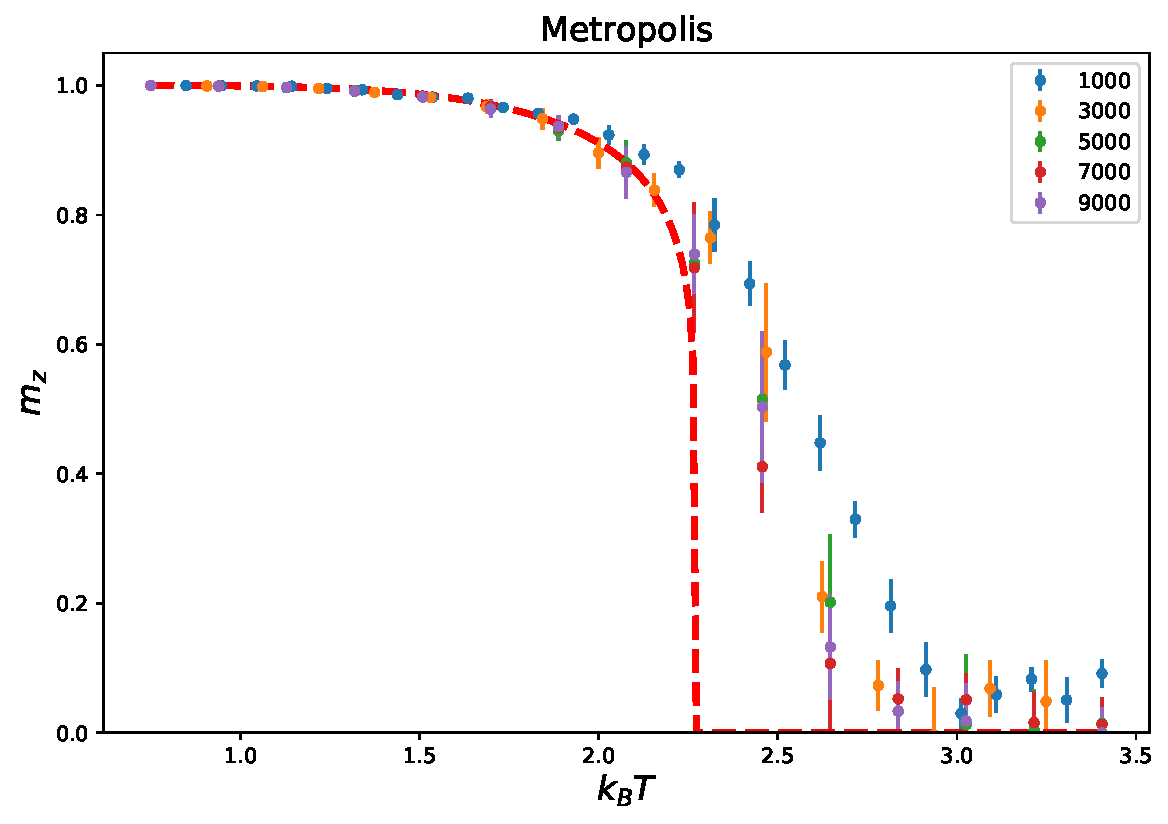
\includegraphics[width=0.8\linewidth]{Figures/metropolis_relax_dependence.pdf}
    \caption{Magnetisation with respect to temperature. Here $k_B=1$, $J=1$ and $h=0$. Red dashed curve corresponds to exact analytical result for an infinite system. Different curves correspond to different relaxation times. Both cases were evaluated for $265$ points. Data was further decreased by data blocking error calculation.}
    \label{fig:relax_dep}
\end{figure}
\subsection{\label{subsec:physicalquantities}Physical quantities}

Physical quantities are not-analytical around the critical temperature. For the quantities discussed here, a power law is followed in this region. The specific heat and the magnetic susceptibility where calculated according to Eqn.\ \ref{eqn:specificheat} and Eqn.\ \ref{eqn:susceptibility}, respectively. The results for each one as a function of temperature for different system sizes are presented in Fig.\ \ref{fig:cv} and Fig.\ \ref{fig:susc}, respectively. 

\begin{figure}[H]
    \centering
    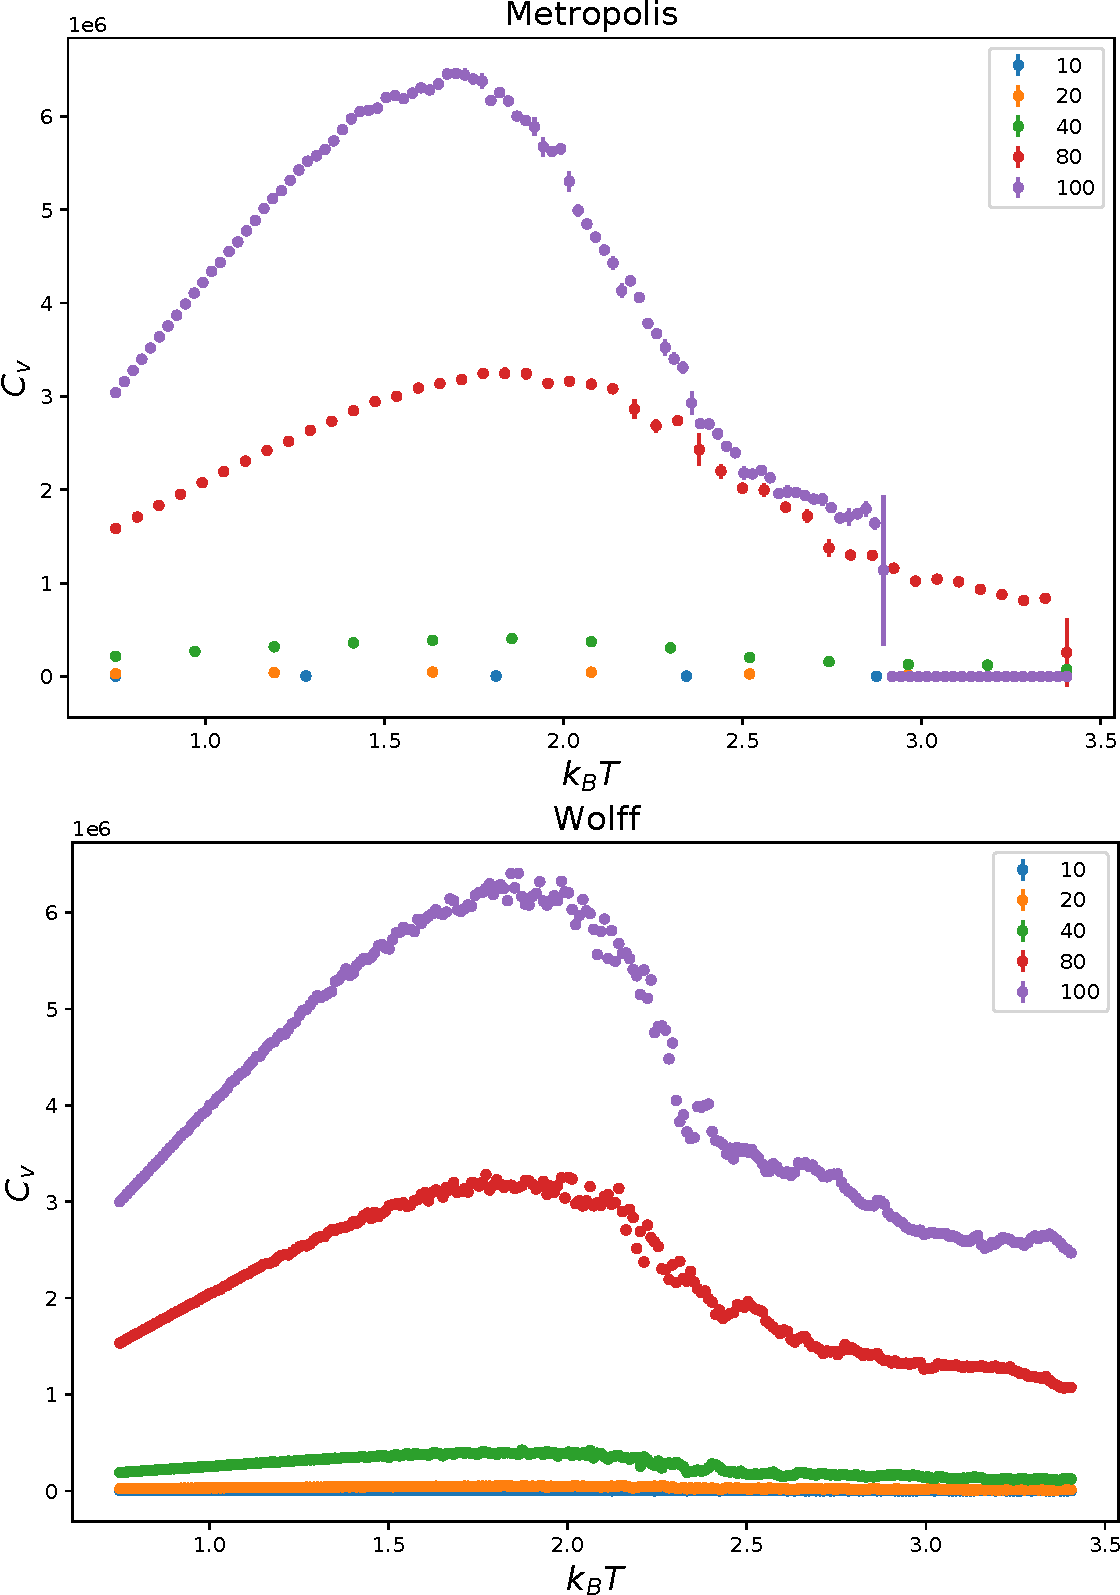
\includegraphics[width=0.8\linewidth]{Figures/cv.pdf}
    \caption{Specific heat with respect to temperature for different system sizes. Here $k_B=1$, $J=1$ and $h=0$. Different curves correspond to different system sizes, i.e. $N$. Both cases were evaluated for $265$ points. Data was further decreased by data blocking error calculation. (Top): Metropolis algorithm with $6000$ relaxation steps. (Bottom): Wolff algorithm with $10$ relaxation steps. Error is too small to be observed.}
    \label{fig:cv}
\end{figure}

For the specific heat, one can observe that the shape is preserved for both algorithms. The height of the divergence at the critical temperature depends on the system size. For the Wolff algorithm (lower panel), there are many more data points than for the Metropolis algorithm (upper panel). Also, data generated by Metropolis overlaps for different system sizes. This does not occur for the Wolff algorithm. 

For the magnetic susceptibility, one can observe significant differences when comparing the data generated by Metropolis and Wolff algorithm. First, for the Wolff algorithm (lower panel) one observes that the position of the divergence is the same regarding the system size. On the contrary, for the Metropolis algorithm (upper panel) the divergence is centred at different temperatures for different system sizes. As expected, for larger sizes, the divergence goes towards the critical temperature.

One can observe that for the Metropolis algorithm, the data sharply goes to zero after reaching the critical temperature. However, this range is extended inversely proportional to the system size. For the Wolff algorithm, this feature is not observed. Instead, one finds a smooth decay from the divergence. 
\begin{figure}[H]
    \centering
    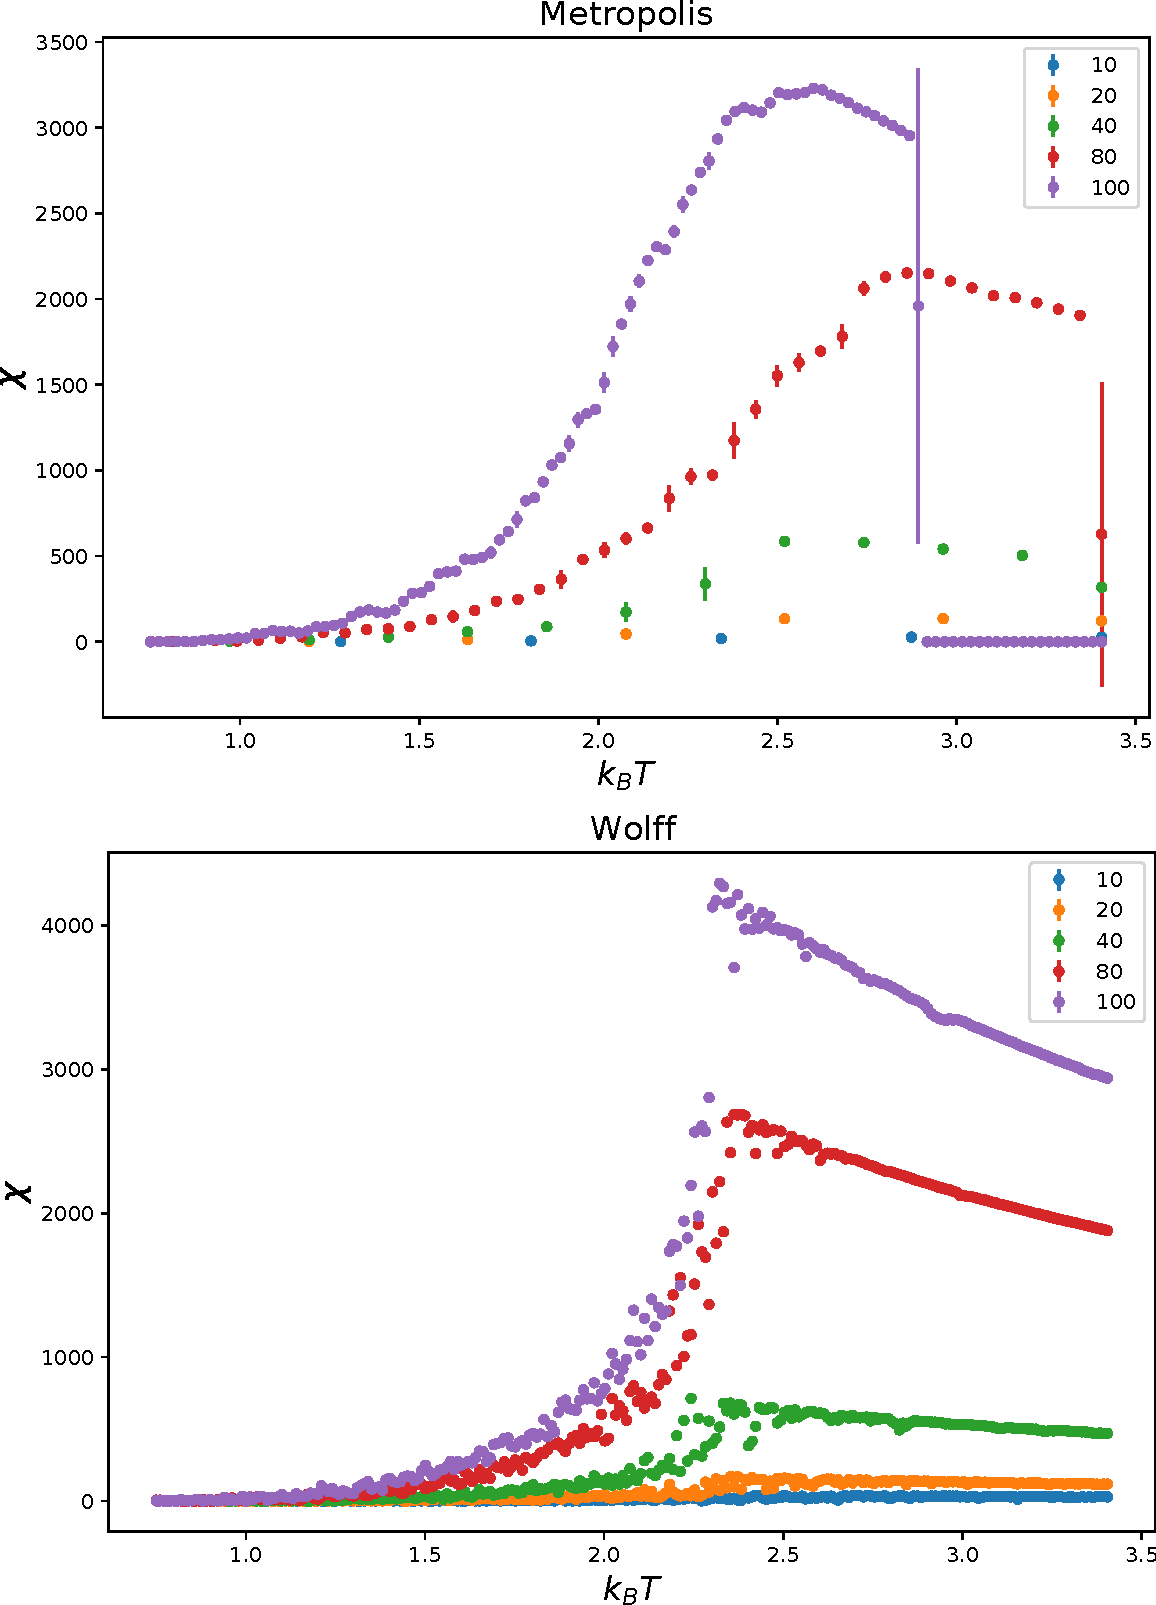
\includegraphics[width=0.8\linewidth]{Figures/susc.pdf}
    \caption{Magnetic susceptibility with respect to temperature for different system sizes. Same parameter configuration as in previous results is used here.}
    \label{fig:susc}
\end{figure}





\subsection{\label{subsec:criticalexponents}Critical exponents}
To model the non-analytic behaviour of the physical quantities around the critical temperature, we fitted our simulated results with a power law decay in order to extract the critical exponents of the system. These results can be compared with the exact analytical results \cite{PhysRev.65.117}. 

\begin{table}[h!]
\centering
\begin{tabular}{||c | c | c | c | c||} 
 \hline
 Exponent & Exact & Metropolis & Wolff & Error \\ [0.5ex] 
 \hline\hline
 $\alpha$ & 0 & 2.813 $\pm$ 0.02 & 2.324 $\pm$ 0.01 &  \\ 
 $\beta$ & 1/8$\approx$0.125 & 0.404 $\pm$ 0.003 & 0.394 $\pm$ 0.001 & 30.94\% \\
 $\gamma$ & 7/4$\approx$ 1.75 & 1.522$\pm$ 0.003 & 1.251$\pm$ 0.006 &  14.98\%\\
 \hline
\end{tabular}
\caption{Critical exponents for the specific heat($\alpha$), magnetisation($\beta$) and magnetic susceptibility($\gamma$) taken from results shown in Fig.\ \ref{fig:cv}, \ref{fig:size_dep}, and \ref{fig:susc}, respectively. The case with the largest lattice ($N=100$) was fitted to a power law decaying function given by $f(t,l)=t^{-l}$ where $t$ is the reduced temperature, and $l$ is the critical exponent to be fitted. For the magnetisation, $l,t\rightarrow -l,-t$ in $f(t,l)$. Errors in the right column are calculated with respect to Metropolis results.}
\label{table:1}
\end{table}
 In Table \ref{table:1} the results of the fitted critical exponents are presented. One can observe that two of them have an error that is below $\sim31\%$. The exponent for the specific heat is quite far from the theory prediction.
\subsection{\label{subsec:phasediagram}Phase diagram}

Using Metropolis algorithm, we began from a lattice with randomly aligned spins and slowly raised (i.e.\ relaxation steps of 2000) the temperature $T/T_C$ from 0 to a target value while also sweeping through the possible values for the external magnetic field $h\in(-1,1)$. The results of this simulation sweep can be seen in Fig.\ \ref{fig:phasediagram}. Since the result was generated using the Metropolis algorithm, we expect the magnetisation to not drop to zero at exactly $T/T_C=1$ but slightly higher, which is indeed what we observe.

\begin{figure}[H]
    \centering
    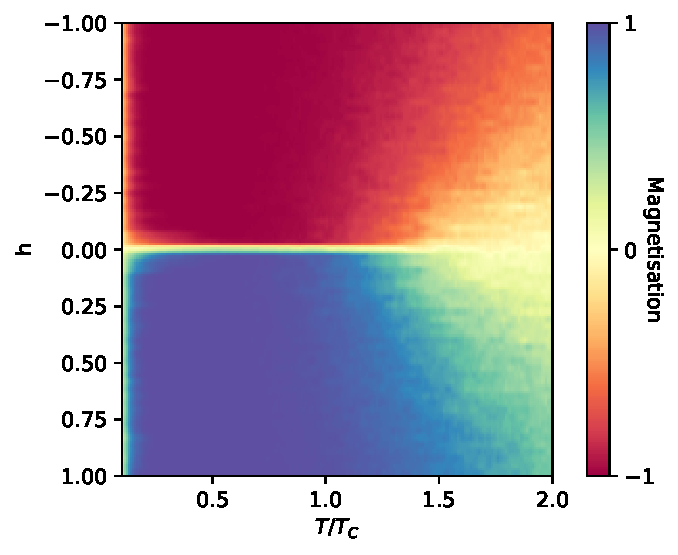
\includegraphics[width=0.9\linewidth]{Figures/phase_diagram.pdf}
    \caption{Phase diagram of the 2D square lattice Ising model using the Metropolis algorithm. The parameters are: $L=50$, $J=1$ and relaxation steps $=2000$.}
    \label{fig:phasediagram}
\end{figure}

Unfortunately, the Wolff algorithm which we implemented does not support varying external magnetic fields, thus there is no corresponding result generated by the Wolff algorithm.

\subsection{\label{subsec:benchmark}Performance}
In this section we study and compare the performance of the Metropolis algorithm and Wolff algorithm. Since the way that each of the algorithm work is fundamentally different (i.e.\ the former flips a single spin while the latter flips an entire cluster in a single iteration), it is crucial that a proper benchmarking procedure is designed so that we can compare them and retrieve relevant insights.

To study the performance of the two algorithms, we measured the time needed to run them starting from a completely positive spin lattice until the absolute average magnetisation of the corresponding systems reaches a threshold value, which we define as $\varepsilon=0.1$. We repeat this 10 times for each value of temperature $T/T_C$, which we chose to range from 1.2 to 2.0 with 20 data points. Then, we calculate the time average of each of the 10 runs and it is denoted by $\bar t$. The result can be obtained by running \texttt{benchmark.py} and its plot can be seen in Fig.\ \ref{fig:benchmark}. 

We chose this specific $T/T_C$ range in order to accentuate the difference in performance between the Metropolis algorithm and the Wolff algorithm. From Fig.\ \ref{fig:benchmark}, we indeed see that the Metropolis algorithm requires significantly more time to reach an absolute average magnetisation of 0.1 starting from a completely positive spin lattice compared to the Wolff algorithm. On the other hand, the average run-time $\bar t$ for the Wolff algorithm seems to remain constant at $\sim 0.2\mathrm{s}$ with slight fluctuations. This implies that the fact that we are near the criticality regime does not impact the its efficiency. The discrepancy in performance between the two algorithms can be explained by section \ref{sec:ErgodicityandDetailedbalance}.

\begin{figure}[H]
    \centering
    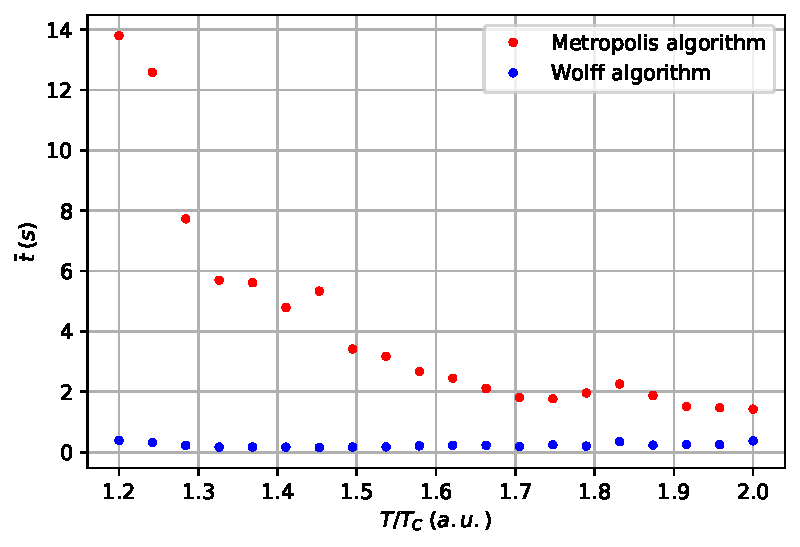
\includegraphics[width=0.9\linewidth]{Figures/benchmark.pdf}
    \caption{Average run-time $\bar t$ for Metropolis algorithm (red) and Wolff algorithm (blue) for the system to reach an absolute average magnetisation of 0.1 beginning from a completely positive spin lattice for varying $T/T_C$. The system size used is $L=64$. The results were obtained on a machine with an \texttt{Intel i5-7200U} CPU.}
    \label{fig:benchmark}
\end{figure}


\section{\label{sec:conclusion}Conclusion}

To conclude, we have studied the system size dependence in section \ref{subsec:systemsizedependence}, where we see that there is an inherent need for the simulation domain to be large such that the physical observables obtained can approach those of analytical results. Then in section \ref{subsec:relaxationsteps}, we showed that ability for the Metropolis algorithm to match the analytical result seems to plateau at high relaxation times, while in section \ref{subsec:systemsizedependence} the Wolff algorithm achieved close proximity to the analytical data. We studied the phase diagram and found expected behaviour in section \ref{subsec:phasediagram}.

We also accessed the physical quantities and the critical exponents in sections \ref{subsec:physicalquantities} and \ref{subsec:criticalexponents}, respectively. We found the expected general behaviour for the physical quantities for varying simulation parameters. However, the general shape of the plots of the specific heat capacity and the magnetic susceptibility seems to deviate from the literature. Furthermore, we found that the critical exponents that we retrieved from the simulations also deviates from the analytical results by a considerable amount. 

From the performance viewpoint, We benchmark-ed our implementation of both the algorithms in section \ref{subsec:benchmark} and found that Wolff algorithm is highly preferred over the Metropolis algorithm especially in the vicinity of the criticality regime.

Finally, despite the considerable deviation of some of the simulation results we obtained, it is no doubt that development in computational physics in simulating ferromagnetism had come a long way and it has become an invaluable tool in studying this phenomena.

\section{\label{sec:Acknowledgements}Acknowledgements}
This work is part of the course AP3082 Computational Physics supported by the Delft University of Technology.

\appendix\label{appendix}
\section{Source code}
The source code can be found in this Gitlab repository: \href{https://gitlab.kwant-project.org/computational_physics/projects/Project-2---Ising_juandaanieel_kwo/}{Gitlab link}.
% Appendix here...

% \section{Second Appendix}
% Appendix here...

% \nocite{*}
\bibliography{references}% Produces the bibliography via BibTeX.
\end{document}